\chapter{Results and Analysis}

The results of the project demonstrate the locomotion of quadrupedal robot, which are pitching, yawing, rolling, and squatting. By adjusting parameters through corresponding custom sliders, a series of actions are obtained through screenshots and merged into figures, where certain text interpretation would be executed. Meanwhile, the analysis would contribute to the comparison among states of joints. The motions of the quadrupedal robot would be dissected respectively.


\section{Squatting}

Squatting, for the quadruped robot, is the action that makes the gravity centre of its main body rise or fall vertically. By pulling the custom slider of squatting to adjust the parameters, a series of actions of the quadruped robot when squatting is shown in Fig.\ref{fig: squatting}.

\begin{figure}[htbp]
    \centering
    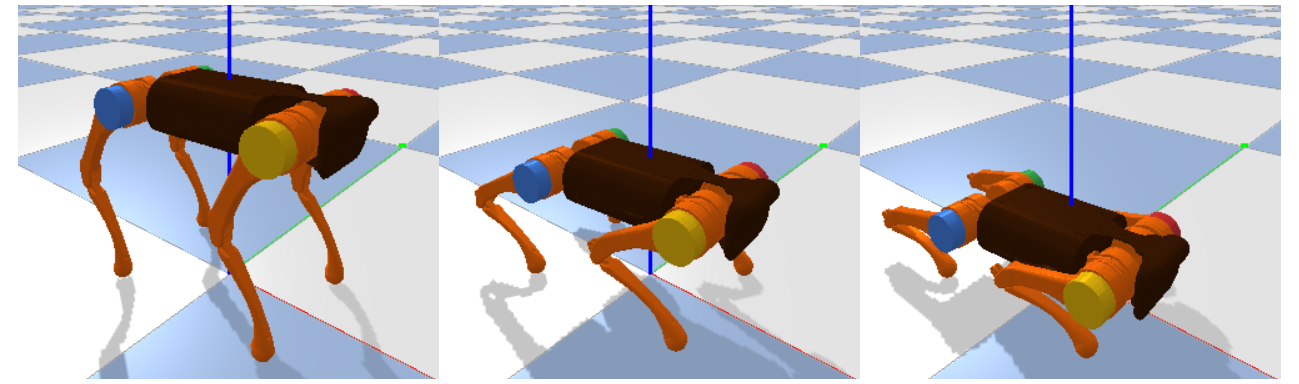
\includegraphics[width=0.8\textwidth]{figures/squatting.png}
    \caption{Squatting}
    \label{fig: squatting}
\end{figure}

In the initial position, the distance from hip joints to toe joints is 270. While the slider of debug parameter was pulled to the left, the distance became smaller, the body of the robot descended vertically. While the slider of debug parameter was pulled to the right, the distance became larger, and the robot's body ascended vertically.

The state of abduction/adduction hip joints would retain the initial state while squatting. The state of flection/extension hip joints and knee joints would change corresponding to the distance from the toe. Judging from the simulation results, the robot's legs were crooked while the robot's trunk moves downward, and were extended while the robot's trunk move upward. The state of knee joints. The state of the knee joints determined the current highest position of the robot, and then the actual position of the robot was adjusted by controlling the state of the hip joint.



\section{Pitching}

Pitching, for the quadruped robot, is the action of rotating about the transverse axis \cite{ref:6DOF}. By pulling the custom slider of pitching to adjust the parameters, a series of actions of the quadruped robot when pitching is shown in Fig.\ref{fig: pitching}.

\begin{figure}[htbp]
    \centering
    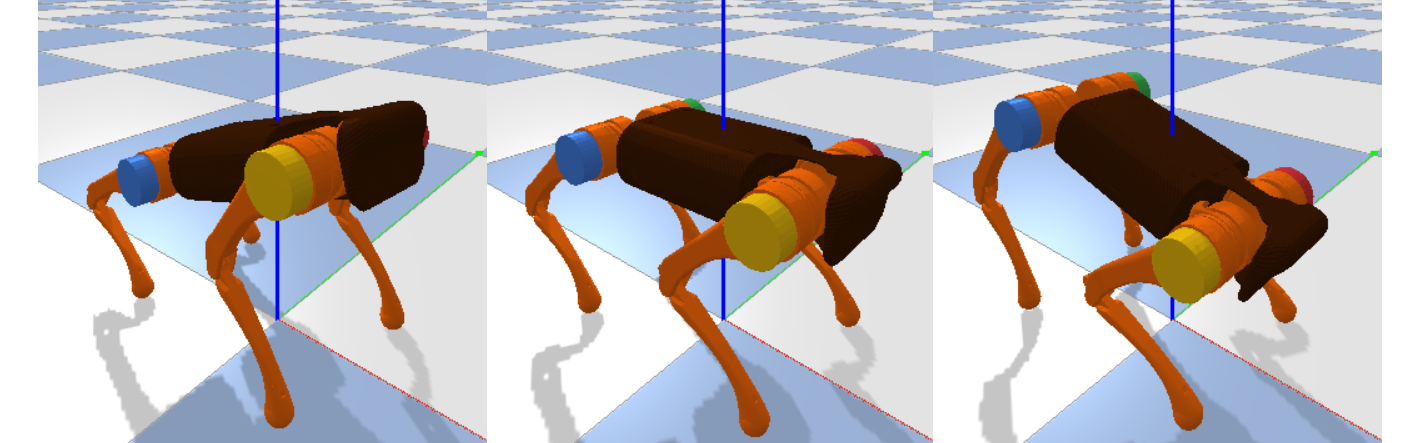
\includegraphics[width=0.8\textwidth]{figures/pitching.png}
    \caption{Pitching}
    \label{fig: pitching}
\end{figure}

In the initial position, the body of the quadruped robot remained horizontal, which means that the pitch angle was 0. While the slider of debug parameter was pulled to the left, the pitch angle became negative, and the robot's body made counterclockwise rotation about the transverse axis. While the slider of debug parameter was pulled to the right, the pitch angle became positive, and the robot's body made clockwise rotation about the transverse axis.

As mentioned in the method, the motion of the robot body only occurs in the plane perpendicular to the transverse axis. Therefore, the variations of joints' states between the left and right legs are consistent, unilateral legs need to be evaluated in the analysis. Compared to the motions of yawing and rolling, the motion of pitching is more straightforward, because the state of abduction/adduction hip joints would retain the initial state. However, in the process of pitching, the state of flection/extension hip joints and knee joints would change with the flection or extension of the legs. While the legs were extended, the calves rotated clockwise, from the left perspective, relative to the knee joints., the thighs rotated counterclockwise, from the left perspective, relative to the flection/extension hip joints. While the legs were crooked, the calves rotated counterclockwise, from the left perspective, relative to the knee joints, the thighs rotated clockwise, from the left perspective, relative to the flection/extension hip joints.


\section{Yawing}

Yawing, for the quadruped robot, is the action of rotating about the normal axis \cite{ref:6DOF}. By pulling the custom slider of squatting to adjust the parameters, a series of actions of the quadruped robot when yawing are shown in Fig.\ref{fig: yawing}.

\begin{figure}[htbp]
    \centering
    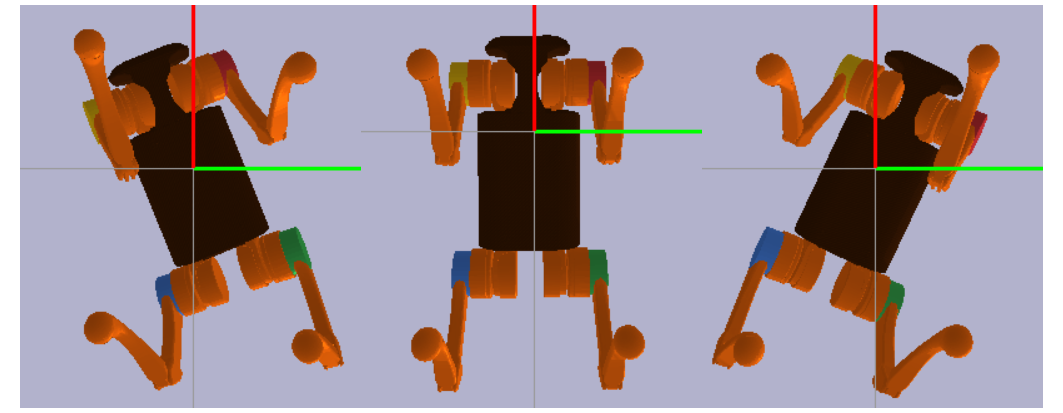
\includegraphics[width=0.8\textwidth]{figures/yawing.png}
    \caption{Yawing}
    \label{fig: yawing}
\end{figure}


For the sake of observing the locomotion of the quadruped robot more intuitively, we chose the bottom view as the observation view in the screenshots of yawing. In the initial position, the body of the quadruped robot was parallel to the longitudinal axis, which means that the yaw angle was 0. While the slider of debug parameter was pulled to the left, the yaw angle became negative, and the robot's body made counterclockwise rotation about the normal axis. While the slider of debug parameter was pulled to the right, the yaw angle became positive, and the robot's body made clockwise rotation about the normal axis.

It can be seen that the leg state of the robot is diagonally symmetrical, that is, the joints' state of the front-left leg is similar to that of the hind-right leg, and the joints' state of the front-right leg is similar to that of the hind-left leg. While the robot yawing to right, the front legs rotated counterclockwise, and the hind legs rotated clockwise, from the front perspective, relative to the abduction/adduction hip joints.The front-right leg and hind-left leg were crooked. The front-left leg and hind-right leg were extended. The state of these joints is actually similar to the motion of leg joints in squatting.


\section{Rolling}

Rolling, for the quadruped robot, is the action of rotating about the longitudinal axis \cite{ref:6DOF}. By pulling the custom slider of squatting to adjust the parameters, a series of actions of the quadruped robot when rolling are shown in Fig.\ref{fig: rolling}.

\begin{figure}[htbp]
    \centering
    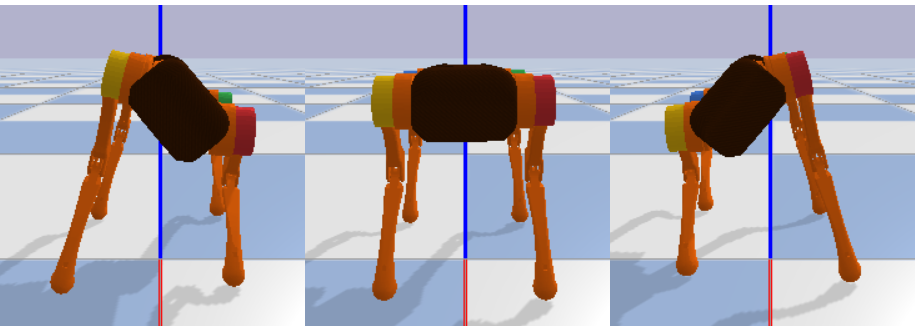
\includegraphics[width=0.8\textwidth]{figures/rolling.png}
    \caption{Rolling}
    \label{fig: rolling}
\end{figure}

For the sake of observing the locomotion of the quadruped robot more intuitively, we chose the front view as the observation view in the screenshots of rolling. In the initial position, the heights of the left and right hip joints from the ground are the same, which means that the roll angle was 0. While the slider of debug parameter was pulled to the left, the roll angle became negative, and the robot's body made clockwise rotation about the longitudinal axis. While the slider of debug parameter was pulled to the right, the roll angle became positive, and the robot's body made counterclockwise rotation about the longitudinal axis.

The change in the joints' state of rolling is similar to pitching, except that the leg state of the robot is left and right symmetrical. While the robot pitched clockwise, the front legs rotated counterclockwise, and the hind legs rotated clockwise, from the front perspective, relative to the abduction/adduction hip joints. The right-side legs would be extended and the left-side legs would be crooked.

